\documentclass[10pt,a4paper]{article}

\usepackage[utf8]{inputenc}
\usepackage[T1]{fontenc}
\usepackage[top=1.0cm,bottom=1.0cm,left=1.4cm,right=1.4cm]{geometry}
\usepackage[expansion=false]{microtype}
\usepackage{amsmath,amssymb}
\usepackage{booktabs}
\usepackage{tabularx}
\usepackage{array}
\usepackage{graphicx}
\usepackage{xcolor}
\usepackage{enumitem}
\usepackage{float}
\usepackage{caption}
\usepackage[hidelinks]{hyperref}

\setlength{\columnsep}{0.6cm}
\setlist{nosep}
\setlength{\abovecaptionskip}{3pt}
\setlength{\belowcaptionskip}{3pt}
\setlength{\textfloatsep}{6pt plus 2pt minus 2pt}
\setlength{\floatsep}{6pt plus 2pt minus 2pt}
\setlength{\intextsep}{6pt plus 2pt minus 2pt}

% Helper macro for visible placeholders to fill after running experiments
\newcommand{\placeholder}[1]{\textcolor{blue!70!black}{\texttt{[#1]}}}

\title{\textbf{Evaluating Lightweight Vision-Language and OCR Models on Occluded Document Images}}
\author{
    Trinh Vo Nam Kiet \quad 24125013 \\
    APCS 24A01 HCMUS --- CS418 \\
    \small\url{https://github.com/namkiet/CS418_Lab1}
}
\date{}

\begin{document}
\maketitle

\begin{abstract}
This report benchmarks 5 pretrained lightweight models---spanning multimodal Vision-Language Models (Florence-2-base, PaddleOCR-VL) and dedicated OCR pipelines (RapidOCR/PP-OCRv6, Tesseract v5.5, EasyOCR 1.7.2)---on the 3,000-page Occluded Pages Restoration Benchmark (OPRB) test evaluation subset under a strictly zero-shot setting. We evaluate character- and word-level accuracy (CER, WER), order-insensitive token F1, robustness across text-region and non-text-region occlusions as well as occlusion types and densities, and per-page inference latency to analyze the trade-offs between compact generative VLMs and dedicated OCR engines for occluded document recognition.
\end{abstract}

\section{Introduction}
\label{sec:intro}

Optical Character Recognition (OCR) on real-world scanned and photographed documents frequently degrades in the presence of physical or digital occlusions such as ink marks, scribbles, stamps, dust, and correction marks. While lightweight Vision-Language Models (VLMs) and dedicated OCR pipelines offer strong zero-shot text extraction capabilities, their relative robustness to partial text obscuration and their computational efficiency remain important practical trade-offs.

In this assignment, we benchmark 5 pretrained lightweight models---spanning both multimodal VLMs and dedicated OCR models---on the Occluded Pages Restoration Benchmark (OPRB) test set. Following the evaluation protocol, all models are evaluated strictly in a zero-shot setting using their pretrained weights without any training or fine-tuning on OPRB. We compare recognition accuracy, robustness across text-region and non-text-region occlusions, error patterns across occlusion types, and inference latency to identify the most suitable models for occluded document recognition.

\section{Dataset Statistics}
\label{sec:dataset}

We evaluate on the \textbf{OPRB test split}, selecting the \textbf{3,000-page} evaluation subset consisting of:
\begin{itemize}
    \item \textbf{Text-region occlusions (\texttt{test/text/img/}):} the first 2,000 pages where occlusions directly overlap textual content.
    \item \textbf{Non-text-region occlusions (\texttt{test/nontext/img/}):} the first 1,000 pages where occlusions appear outside primary text blocks (e.g., margins or figures).
\end{itemize}

Ground-truth transcripts are extracted exclusively from the corresponding \texttt{gt/} annotation files (tab-separated DocBank records) by reading the token column in row order. Clean page images (\texttt{img\_gt/}) and occlusion masks (\texttt{annots/}) are never provided to any model. Table~\ref{tab:dataset} summarizes the subset composition and occlusion metadata parsed from image filenames.

\begin{table}[H]
    \centering
    \caption{OPRB test evaluation subset statistics (3,000 images).}
    \label{tab:dataset}
    \footnotesize
    \begin{tabularx}{\columnwidth}{lrr>{\raggedright\arraybackslash\hsize=0.98\hsize}X>{\raggedright\arraybackslash\hsize=1.02\hsize}Xc}
        \toprule
        \textbf{Subset} & \textbf{Pages} & \textbf{Share} & \textbf{Observed Occlusion Types} & \textbf{Densities} & \textbf{Avg.\ Words} \\
        \midrule
        \texttt{text}    & 2,000 & 66.7\% & Black\_Ink (1,000), Sim (1,000) & 0.5\%, 1.0\%, 2.0\%; Natural: Sim & 556.1 \\
        \texttt{nontext} & 1,000 & 33.3\% & Black\_Ink (537), Sim (423), Dust (40) & 0.5\%, 1.0\%, 2.0\%; Natural: Sim, Dust & 755.3 \\
        \midrule
        \textbf{Total}   & \textbf{3,000} & \textbf{100\%} & 3 types: Black\_Ink, Sim, Dust & 0.5\%, 1.0\%, 2.0\% + natural overlays & 622.5 \\
        \bottomrule
    \end{tabularx}
\end{table}

\section{Model Descriptions}
\label{sec:models}

We evaluate 5 lightweight models using official pretrained weights without test-time adaptation:

\begin{itemize}
    \item \textbf{Florence-2-base (VLM):} Multimodal foundation model ($\approx$232M parameters) by Microsoft, combining a DaViT vision backbone with transformer encoder-decoder, evaluated in FP16 with \texttt{"<OCR>"} prompt (\texttt{num\_beams=1}, \texttt{max\_new\_tokens=1024}).
    \item \textbf{PaddleOCR-VL (VLM):} Compact vision-language OCR model ($\approx$0.9B parameters) by PaddlePaddle, evaluated in FP16 with \texttt{"OCR:"} prompt (\texttt{batch\_size=8}, \texttt{max\_new\_tokens=2048}, \texttt{repetition\_penalty=1.15}, \texttt{no\_repeat\_ngram\_size=6}).
    \item \textbf{RapidOCR / PP-OCRv6 (OCR):} Efficient ONNX OCR pipeline ($\approx$15M parameters, $\approx$17\,MB) pairing a DBNet detector with an SVTR/MobileNet text recognizer in FP32 precision.
    \item \textbf{Tesseract v5.5 / pytesseract (OCR):} Google's LSTM OCR engine ($\approx$25M parameters, $\approx$15\,MB) running with Page Segmentation Mode 3 (\texttt{--psm 3}) and OCR Engine Mode 3 (\texttt{--oem 3}).
    \item \textbf{EasyOCR 1.7.2 / PyTorch (OCR):} Two-stage OCR system ($\approx$40M parameters, $\approx$85\,MB) combining CRAFT text detection with a ResNet-LSTM-CTC recognizer (batch size 32).
\end{itemize}

\paragraph{Inference Protocol \& Hardware Disparity.} All VLM runs employ deterministic decoding (\texttt{do\_sample=False}) with Unicode NFKC normalization, whitespace collapsing, and casefolding. Florence-2-base and PaddleOCR-VL were evaluated on cloud \textbf{Kaggle dual Tesla T4 GPUs} ($2\times 15$\,GB), RapidOCR and EasyOCR ran on a \textbf{local CUDA GPU} (NVIDIA RTX 3050 Laptop GPU, 6\,GB), and Tesseract ran on \textbf{local CPU} (16 threads). Latency metrics reflect these distinct compute backends, whereas character- and word-level accuracy remain directly comparable.

\begin{table}[H]
    \centering
    \caption{Summary of evaluated lightweight models.}
    \label{tab:models}
    \footnotesize
    \renewcommand{\arraystretch}{0.85}
    \begin{tabularx}{\columnwidth}{l c c c >{\raggedright\arraybackslash}X}
        \toprule
        \textbf{Model} & \textbf{Type} & \textbf{Params / Size} & \textbf{Precision} & \textbf{Execution Environment} \\
        \midrule
        Florence-2-base & VLM & 232M / 460\,MB & FP16 & Kaggle GPU ($2\times$ Tesla T4) \\
        PaddleOCR-VL & VLM & 0.9B / 1.8\,GB & FP16 & Kaggle GPU ($2\times$ Tesla T4) \\
        RapidOCR (PP-OCRv6) & OCR & 15M / 17\,MB & FP32 & Local GPU (RTX 3050 CUDA) \\
        Tesseract v5.5 & OCR & 25M / 15\,MB & INT8/FP32 & Local CPU (16 threads) \\
        EasyOCR 1.7.2 & OCR & 40M / 85\,MB & FP32 & Local GPU (RTX 3050 CUDA) \\
        \bottomrule
    \end{tabularx}
\end{table}

\section{Experimental Results}
\label{sec:results}

We report macro-averaged per-page metrics across all successfully processed test images: Character Error Rate (\textbf{CER} $\downarrow$), Word Error Rate (\textbf{WER} $\downarrow$), order-insensitive bag-of-words token \textbf{Precision}, \textbf{Recall}, and \textbf{F1} ($\uparrow$), and average \textbf{Inference Time} (seconds/image $\downarrow$).

\subsection{Quantitative Results}
Table~\ref{tab:overall_results} presents overall results on the 3,000-page OPRB test subset. \textbf{RapidOCR (PP-OCRv6)} attains best overall accuracy, achieving lowest CER ($0.3317$), lowest WER ($0.4283$), and highest token F1 ($0.7678$). \textbf{PaddleOCR-VL} ranks second overall (CER $0.4194$, WER $0.5886$, F1 $0.6765$), outperforming \textbf{Tesseract v5.5} (CER $0.4768$, F1 $0.5194$) and \textbf{EasyOCR} (CER $0.5930$, F1 $0.3556$). While \textbf{Florence-2-base} achieves fast inference ($0.82$\,s/img on dual T4 GPUs), its accuracy degrades severely (CER $1.0415$, Recall $0.2730$) due to an architectural bottleneck: its generation output is strictly capped at $1024$ tokens (\texttt{max\_new\_tokens=1024}). Because OPRB pages average $622.5$ words (often exceeding $1,000$--$1,500$ subword tokens), generation truncates mid-page; ungenerated tokens are penalized as deletions, mechanically driving CER $>1.0$ and deflating Recall.

\begin{table}[H]
    \centering
    \caption{Overall macro-averaged performance on the OPRB test evaluation subset (3,000 images).}
    \label{tab:overall_results}
    \footnotesize
    \renewcommand{\arraystretch}{0.85}
    \begin{tabular}{lccccccc}
        \toprule
        \textbf{Model} & \textbf{Category} & \textbf{CER $\downarrow$} & \textbf{WER $\downarrow$} & \textbf{Precision $\uparrow$} & \textbf{Recall $\uparrow$} & \textbf{F1 $\uparrow$} & \textbf{Time (s/img) $\downarrow$} \\
        \midrule
        Florence-2-base & VLM & 1.0415 & 0.8008 & 0.5559 & 0.2730 & 0.3519 & \textbf{0.82} \\
        PaddleOCR-VL & VLM & 0.4194 & 0.5886 & 0.7721 & 0.6471 & 0.6765 & 9.13 \\
        RapidOCR (PP-OCRv6) & OCR & \textbf{0.3317} & \textbf{0.4283} & \textbf{0.8691} & \textbf{0.7072} & \textbf{0.7678} & 0.84 \\
        Tesseract v5.5 & OCR & 0.4768 & 0.6451 & 0.6431 & 0.4556 & 0.5194 & 0.95 \\
        EasyOCR 1.7.2 & OCR & 0.5930 & 0.8232 & 0.4426 & 0.3066 & 0.3556 & 2.57 \\
        \bottomrule
    \end{tabular}
\end{table}

\subsection{Text vs.\ Non-Text Region Occlusions}
Table~\ref{tab:region_comparison} compares model performance on \texttt{text} (2,000 pages) versus \texttt{nontext} (1,000 pages) occlusions. Models exhibit distinct degradation patterns: RapidOCR achieves higher token F1 on text occlusions ($0.7854$) than on non-text occlusions ($0.7326$), though non-text corruptions produce higher CER ($0.4646$ vs $0.2652$) due to non-text background artifacts being falsely detected as text tokens. PaddleOCR-VL ($0.7013$ vs.\ $0.6268$ F1), Tesseract, and EasyOCR degrade similarly, while Florence-2 remains constrained by generation truncation across both subsets.

\begin{table}[H]
    \centering
    \caption{Performance comparison by occlusion region (\texttt{text} vs.\ \texttt{nontext}).}
    \label{tab:region_comparison}
    \footnotesize
    \renewcommand{\arraystretch}{0.85}
    \begin{tabular}{lcccc}
        \toprule
        & \multicolumn{2}{c}{\textbf{\texttt{text} (2,000)}} & \multicolumn{2}{c}{\textbf{\texttt{nontext} (1,000)}} \\
        \cmidrule(lr){2-3} \cmidrule(lr){4-5}
        \textbf{Model} & \textbf{CER $\downarrow$} & \textbf{F1 $\uparrow$} & \textbf{CER $\downarrow$} & \textbf{F1 $\uparrow$} \\
        \midrule
        Florence-2-base & 1.0265 & 0.3640 & 1.0714 & 0.3277 \\
        PaddleOCR-VL & 0.3562 & 0.7013 & 0.5457 & 0.6268 \\
        RapidOCR (PP-OCRv6) & \textbf{0.2652} & \textbf{0.7854} & \textbf{0.4646} & \textbf{0.7326} \\
        Tesseract v5.5 & 0.4183 & 0.5393 & 0.5939 & 0.4796 \\
        EasyOCR 1.7.2 & 0.5619 & 0.3718 & 0.6553 & 0.3232 \\
        \bottomrule
    \end{tabular}
\end{table}

\subsection{Robustness Analysis}
We group recognition errors by occlusion type and density across evaluated models. Across all corruptions, \textbf{RapidOCR} demonstrates the highest robustness (WER $0.4190$--$0.4583$), followed by \textbf{PaddleOCR-VL} ($0.5730$--$0.6644$), \textbf{Tesseract} ($0.6441$--$0.6780$), \textbf{Florence-2} ($0.7950$--$0.8071$), and \textbf{EasyOCR} ($0.8228$--$0.8271$). Natural simulations (\texttt{Sim}) yield lower WER ($0.4190$ on RapidOCR) than opaque streaks (\texttt{Black\_Ink}, $0.4362$) and scattered noise (\texttt{Through\_Dust}, $0.4583$), whereas PaddleOCR-VL performs slightly better on \texttt{Black\_Ink} ($0.5730$) than \texttt{Sim} ($0.6034$) and \texttt{Through\_Dust} ($0.6644$). Scaling occlusion density steadily degrades performance: on \texttt{Black\_Ink}, RapidOCR WER climbs from $0.4145$ ($0.5\%$) to $0.4288$ ($1.0\%$) and $0.4654$ ($2.0\%$), Tesseract WER increases from $0.6233$ to $0.6752$, and PaddleOCR-VL rises from $0.5583$ ($0.5\%$) to $0.6171$ ($2.0\%$).

\begin{figure}[H]
    \centering
    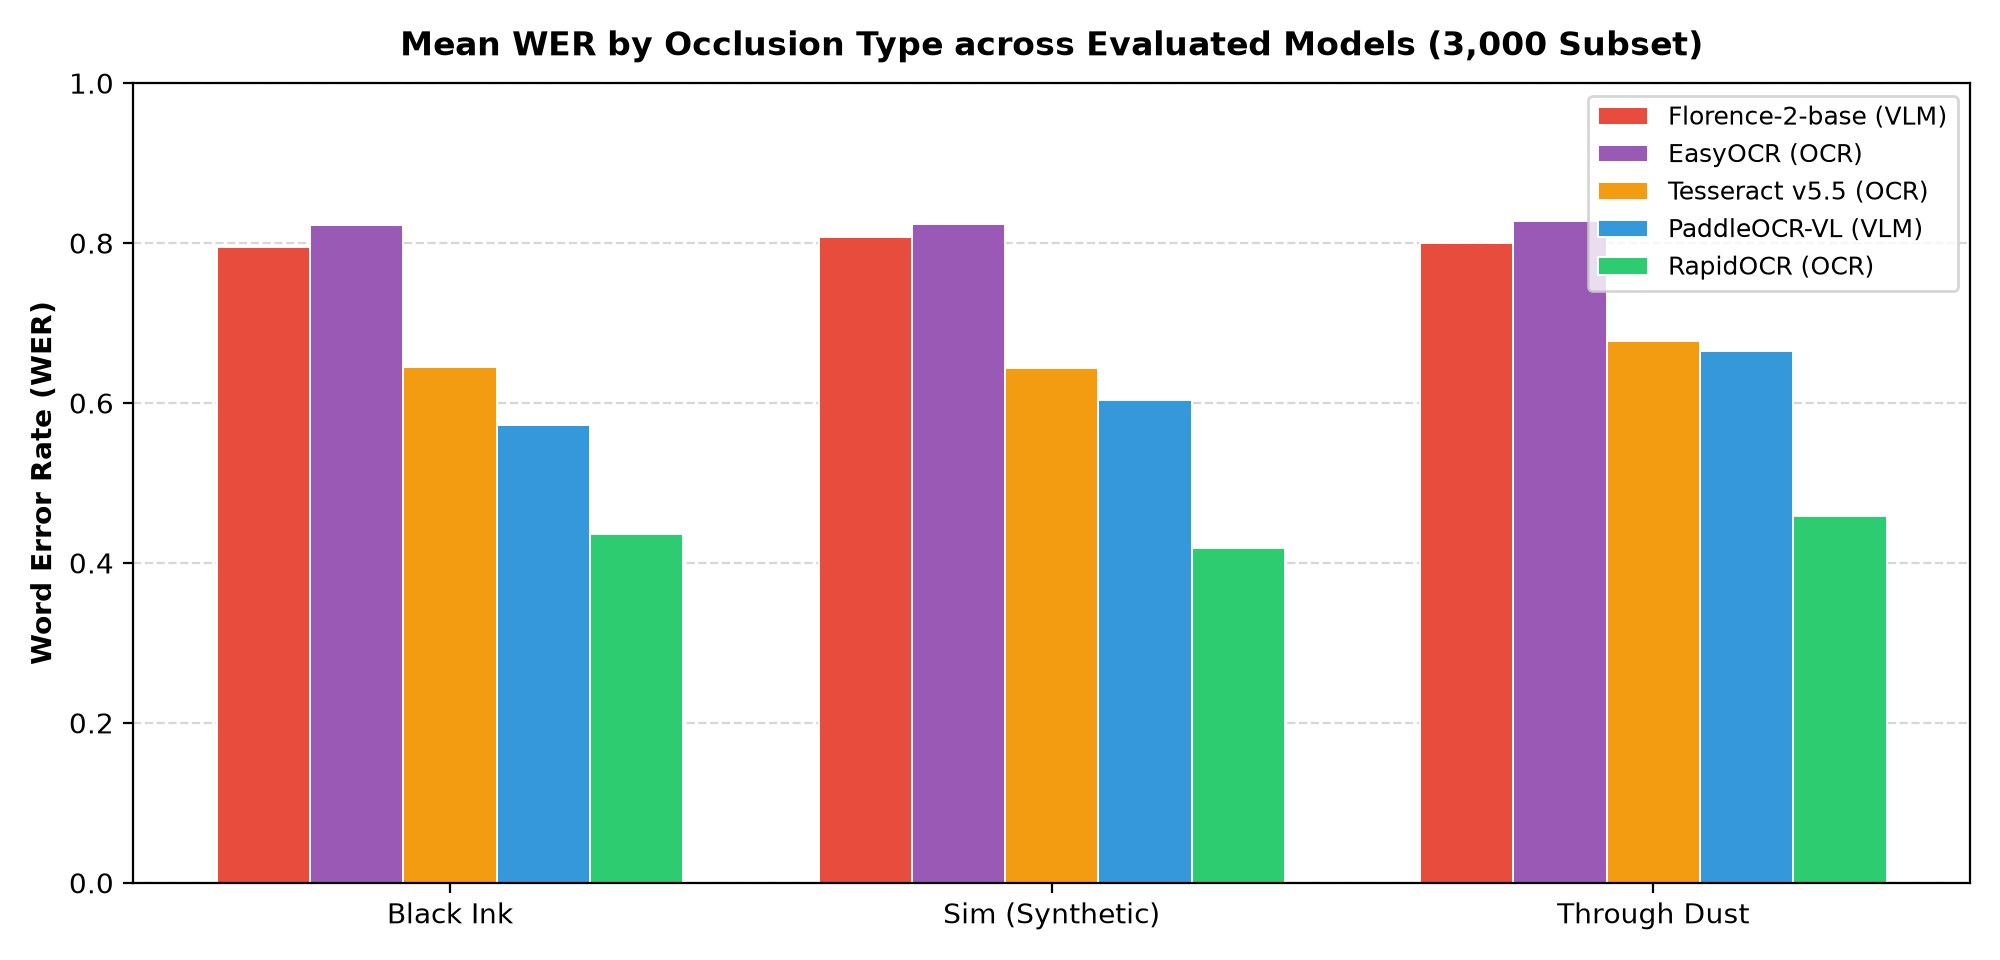
\includegraphics[width=0.75\columnwidth]{figures/wer_by_occlusion_type.png}
    \caption{Mean WER across occlusion types on OPRB test images.}
    \label{fig:occlusion_types}
\end{figure}

\subsection{Qualitative Examples}
We examine representative test predictions from \url{per_image_results.csv} illustrating key recognition behaviors under different corruptions:
\begin{itemize}[leftmargin=*,itemsep=2pt]
    \item \textbf{Successful Robustness (\texttt{spdy\_tr\_0}, \texttt{Black\_Ink}, 1.0\%):} RapidOCR transcribes dense academic text with near-perfect fidelity ($\text{CER}=0.0043$). Bounding box detection traces text lines across ink streaks without fragmentation: \\
    \hspace*{1em}\textbf{GT:} ``\textit{The Effect of Network and Infrastructural Variables on SPDY's Performance...}'' \\
    \hspace*{1em}\textbf{Pred:} ``\textit{The Effect of Network and Infrastructural Variables on SPDY's Performance...}''

    \item \textbf{Omission via Dense Masking (\texttt{paper\_7\_ori}, \texttt{Black\_Ink}, 2.0\%):} Heavy 2.0\% ink streaks obliterate entire text segments ($\text{CER}=0.6972$). The recognizer skips severed words and outputs fragmented characters, causing unavoidable token deletions.

    \item \textbf{Spurious Artifact Insertion (\texttt{paper\_19\_ori}, \texttt{Sim}, nontext):} Non-text chart axes and tick marks in figure regions are falsely detected as alphanumeric sequences ($\text{CER}=1.7050$), inserting hallucinated strings before the actual caption text.
\end{itemize}

\subsection{Efficiency Analysis}
Dedicated OCR pipelines demonstrate exceptional parameter efficiency: \textbf{RapidOCR} operates with only $\approx$15M parameters ($\approx$17\,MB) and processes full pages in $0.84$\,s on a local GPU while attaining best recognition accuracy ($\text{CER}=0.3317$, token $\text{F1}=0.7678$). \textbf{Tesseract v5.5} achieves competitive $0.95$\,s/image processing on a 16-thread CPU. In contrast, \textbf{EasyOCR} ($\approx$40M parameters) requires $2.57$\,s/image even with GPU batching (size 32) and obtains lower F1 ($0.3556$). Among generative VLMs, \textbf{Florence-2-base} ($\approx$232M parameters, $2\times$ Tesla T4) achieves $0.82$\,s/image but suffers from high character error rates ($\text{CER}=1.0415$) because its $1024$-token generation budget truncates lengthy documents. \textbf{PaddleOCR-VL} ($\approx$0.9B parameters, $2\times$ Tesla T4) mitigates truncation with a $2048$-token budget and anti-repetition decoding to reach second-best accuracy ($\text{F1}=0.6765$), but incurs $9.13$\,s/image latency---over $10\times$ slower than RapidOCR. Line-level OCR engines process bounding boxes independently across the whole page canvas without sequence length constraints, making lightweight OCR engines vastly superior in edge document restoration.

\section{Conclusion}
\label{sec:conclusion}

We evaluated 5 lightweight VLMs and OCR engines on the 3,000-image OPRB benchmark subset without fine-tuning. RapidOCR (PP-OCRv6) demonstrated the strongest overall accuracy and efficiency, while the specialized VLM PaddleOCR-VL ranked second and substantially outperformed Tesseract, EasyOCR, and Florence-2-base at the cost of higher inference latency. While non-text corruptions trigger spurious insertions in OCR detectors, text masking imposes unavoidable omissions.

\paragraph{Model Recommendation \& Limitations.} For accuracy-critical transcription under occlusion, \textbf{RapidOCR} (PP-OCRv6) provides the strongest balance of CER/WER and token F1 ($0.7678$), while achieving practical sub-second latency ($0.84$\,s/img on a local GPU). Benchmarking against clean-page annotations penalizes models that refrain from guessing obscured tokens, and row-order concatenation can inflate CER/WER on multi-column layouts.


\end{document}
